\documentclass[11pt,a4paper]{article}
\usepackage[T1]{fontenc}
\usepackage[utf8]{inputenc}
\usepackage[polish]{babel}
\usepackage{amsmath}
\usepackage{amsfonts}
\usepackage[margin=2cm]{geometry} % to change margins
\usepackage{graphicx}
\usepackage[export]{adjustbox} % to adjust graphics to either left or right or center
\author{Kamil Kuczaj}
\title{Sprawozdanie z Laboratorium 2 - Pomiar czasu dynamicznej alokacji pamięci w tablicy dynamicznej.}
\date{\today}
\begin{document}

\maketitle

\section{Wstęp}
Podanym zadaniem był pomiar czasu znajdywania losowego elementu listy typu\textit{string}. Należało wykonać pomiary zapisu: $10^1$, $10^3$, $10^5$, $10^6$ oraz $10^9$ elementow używając różnych metod zmiany rozmiaru pamięci dynamicznej tablicy. W swoim sprawozdaniu porównałem trzy metody:
\begin{list}{•}{}
\item Zwiększanie rozmiaru tablicy \textbf{o 1 element}
\item \textbf{Dwukrotne} zwiększanie rozmiaru
\item \textbf{Trzykrotne} zwiększanie rozmiaru
\end{list}
\smallskip
Każdy pomiar został powtórzony \textbf{50} razy a wyniki zapisane do plików z rozszerzeniem \textit{.csv} i umieszczone w folderze wyniki.\\\\
W sprawozdaniu podążałem za podręcznikiem \textit{\textbf{Google C++ Guide}}, aby mój kod był czytelny oraz podążał za światowym standardem. Sama konstrukcja programu jest modułowa oraz zaimplementowano w nich interfejs.

\section{Specyfikacja komputera}

\begin{center}
	\begin{tabular}{| r | c |}
	\hline
	Wersja kompilatora \textit{g++} & 4.8.4 \\ \hline
	System & Ubuntu 14.04.4 \\ \hline
	Procesor	 & Intel Core i5 2510M 2.3 GHz \\ \hline
	Pamięć RAM & 8 GB DDR3 1600 MHz \\ \hline
	Rozmiar zmiennej \textit{int} & 4 bajty \\ \hline
	\end{tabular}
\end{center}

\section{Pomiary oraz ich interpretacja}

\hspace{4ex}Wykonałem pomiary dla zapisu podanych powyżej ilości elementów wykorzystując i porównując dwie metody. Jedna opierała się na alokacji zwiększając rozmiar tablicy dynamicznej dwukrotnie a druga na zwiększaniu trzykrotnym. Zostały porównane z wynikami metody, która polegała na zwiększaniu rozmiaru tablicy o jeden element.\\

Ilość zajętej pamięci RAM przed pomiarami wynosiła około $1,6$ GB.

\newpage

\begin{table}[h!]
\centering
\label{my-label1}
	\begin{tabular}{| l | c | c | c |}
	\hline
	\textbf{Ilość elementów} & 10 & $10^3$ & $10^5$ \\ \hline
	\textbf{Średnie czasy {[}$\mu s${]} } & 0,12 & 1606,52 &	14424750 \\ \hline
	\textbf{Średnie czasy {[}s{]} } & 0,00000012	& 0,00160652 & 14,42475 \\ \hline
	\end{tabular}
	\caption{Średnie pomiary czasu zapisu przy zwiększaniu rozmiaru tablicy dynamicznej o jeden element. Brak dalszych pomiarów wynika z tego, iż trwały one bardzo długo. Posiadając już te jestem w stanie dowieść, że jest to metoda bardzo nieefektywna.}
\end{table}

\bigskip
\bigskip

\begin{table}[h!]
\centering
\label{my-label2}
	\begin{tabular}{| l | c | c | c | c | c |}
	\hline
	\textbf{Ilość elementów} & 10 & $10^3$ & $10^5$ & $10^6$ & $10^9$ \\ \hline
	\textbf{Średnie czasy {[}$\mu s${]} } & 0,06       & 13,34      & 1345,3    & 10834,8   & 		10035074,2 \\ \hline
	\textbf{Średnie czasy {[}s{]} } & 0,00000006 & 0,00001334 & 0,0013453 & 0,0108348 & 	10,0350742 \\ \hline
	\end{tabular}
	\caption{Średnie pomiary czasu zapisu przy dwukrotnym zwiększaniu rozmiaru tablicy dynamicznej.}
\end{table}

\bigskip
\bigskip

\begin{table}[h!]
\centering
\label{my-label3}
	\begin{tabular}{| l | c | c | c | c | c |}
	\hline
	\textbf{Ilość elementów} & 10 & $10^3$ & $10^5$ & $10^6$ & $10^9$ \\ \hline
	\textbf{Średnie czasy {[}$\mu s${]} } & 0,14 & 10,48 & 1170,72 & 7839,26 & 7814924,6 \\ \hline
	\textbf{Średnie czasy {[}s{]} } & 0,00000014	& 0,00001048	& 0,00117072	 & 0,00783926 & 7,8149246 \\ \hline
	\end{tabular}
	\caption{Średnie pomiary czasu zapisu przy trzykrotnym zwiększaniu rozmiaru tablicy dynamicznej.}
\end{table}

\bigskip
\bigskip

Dane prognoza zostały otrzymane poprzez ustalenie, że wraz ze wzrostem ilości danych proporcjonalne wzrośnie czas ich alokacji - liniowość. Jak widać przy alokacji 10 elementów, spodziewalibyśmy się krótszego czasy alokacji miliona elementów.\\
Natomiast czas alokacji w momencie tysiąca lub stu tysięcy wskazuje, że alokacja pamięci dla dziesięciu zmiennych całkowitych będzie trwać dłużej niż rzeczywisty czas.\\\\
Zobrazowanie tego konceptu zostało zilustrowane przy użyciu programu \textit{LibreOffice Calc} i jest widoczne na następnej stronie.

\newpage

\begin{figure}

	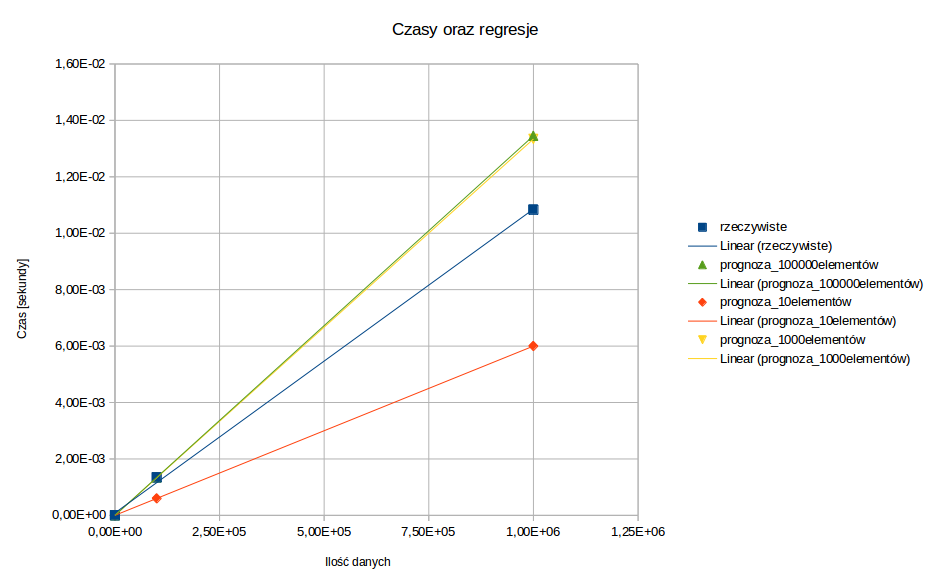
\includegraphics[scale=0.5,left]{../wykresy/CzasyOrazRegresje.png}

\caption{Zobrazowanie wyników pomiaru dla metody dwukrotnego zwiększania rozmiaru tablicy. Najlepiej dopasowuje się tutaj regresja liniowa.}
\end{figure}


\section{Wnioski}

\hspace{4ex} Wyraźnie widać wyższość metody alokacji podwójnej nad metodą zwiększania jej rozmiaru o jeden element. Jednak trzykrotne zwiększanie rozmiaru tablicy pokazuje wyższość, to potrzeba na ten sposób więcej surowców (pamięci fizycznej). Dwukrotne zwiększanie rozmiaru tablicy w zupełności wystarcza.\\
Kilkukrotne zwiększanie rozmiaru tablicy powoduje, że algorytm ten zyskuje złożoność obliczeniową rzędu $n$ w notacji dużego $\Theta$. Natomiast rozszerzanie rozmiaru tablicy metodą dodawania n-elementów powoduje, że złożoność obliczeniowa wzrasta do $n^2$ w notacji dużego $\Theta$.

\end{document}